% =====================================================================
% figF  — R/ggplot2 -> tikzDevice (parallel to ../figures-tex/figF_sequential.tex)
% Canonical-JSON-only. Regenerate: Rscript figures/make_figures_ieee.R
% Provenance (JSON path :: field = plotted value), one line per series:
% SOURCE: results/SEQ_analysis_L12_4stream.json :: per_stream[0].survival_curve[10].frac_survived = 0.5000
% SOURCE: results/SEQ_analysis_L12_4stream.json :: per_stream[0].survival_curve[20].frac_survived = 0.3500
% SOURCE: results/SEQ_analysis_L12_4stream.json :: per_stream[0].survival_curve[30].frac_survived = 0.3667
% SOURCE: results/SEQ_analysis_L12_4stream.json :: per_stream[0].survival_curve[40].frac_survived = 0.2250
% SOURCE: results/SEQ_analysis_L12_4stream.json :: per_stream[0].survival_curve[50].frac_survived = 0.1000
% SOURCE: results/SEQ_analysis_L12_4stream.json :: per_stream[1].survival_curve[10].frac_survived = 0.6000
% SOURCE: results/SEQ_analysis_L12_4stream.json :: per_stream[1].survival_curve[20].frac_survived = 0.3000
% SOURCE: results/SEQ_analysis_L12_4stream.json :: per_stream[1].survival_curve[30].frac_survived = 0.3667
% SOURCE: results/SEQ_analysis_L12_4stream.json :: per_stream[1].survival_curve[40].frac_survived = 0.4000
% SOURCE: results/SEQ_analysis_L12_4stream.json :: per_stream[1].survival_curve[50].frac_survived = 0.1400
% SOURCE: results/SEQ_analysis_L12_4stream.json :: per_stream[2].survival_curve[10].frac_survived = 0.6000
% SOURCE: results/SEQ_analysis_L12_4stream.json :: per_stream[2].survival_curve[20].frac_survived = 0.6000
% SOURCE: results/SEQ_analysis_L12_4stream.json :: per_stream[2].survival_curve[30].frac_survived = 0.7000
% SOURCE: results/SEQ_analysis_L12_4stream.json :: per_stream[2].survival_curve[40].frac_survived = 0.3500
% SOURCE: results/SEQ_analysis_L12_4stream.json :: per_stream[2].survival_curve[50].frac_survived = 0.4200
% SOURCE: results/SEQ_analysis_L12_4stream.json :: per_stream[3].survival_curve[10].frac_survived = 0.4000
% SOURCE: results/SEQ_analysis_L12_4stream.json :: per_stream[3].survival_curve[20].frac_survived = 0.5000
% SOURCE: results/SEQ_analysis_L12_4stream.json :: per_stream[3].survival_curve[30].frac_survived = 0.3333
% SOURCE: results/SEQ_analysis_L12_4stream.json :: per_stream[3].survival_curve[40].frac_survived = 0.1750
% SOURCE: results/SEQ_analysis_L12_4stream.json :: per_stream[3].survival_curve[50].frac_survived = 0.3600
% SOURCE: results/SEQ_analysis_L12_4stream.json :: per_stream[0].position_fragility.rho_position_vs_survival = 0.3118
% SOURCE: results/SEQ_analysis_L12_4stream.json :: per_stream[1].position_fragility.rho_position_vs_survival = 0.2017
% SOURCE: results/SEQ_analysis_L12_4stream.json :: per_stream[2].position_fragility.rho_position_vs_survival = 0.4816
% SOURCE: results/SEQ_analysis_L12_4stream.json :: per_stream[3].position_fragility.rho_position_vs_survival = 0.5139
% SOURCE: results/SEQ_analysis_L12_4stream.json :: pooled.position_fragility.rho_position_vs_survival = 0.3716
% =====================================================================
% !TEX encoding = UTF-8 Unicode
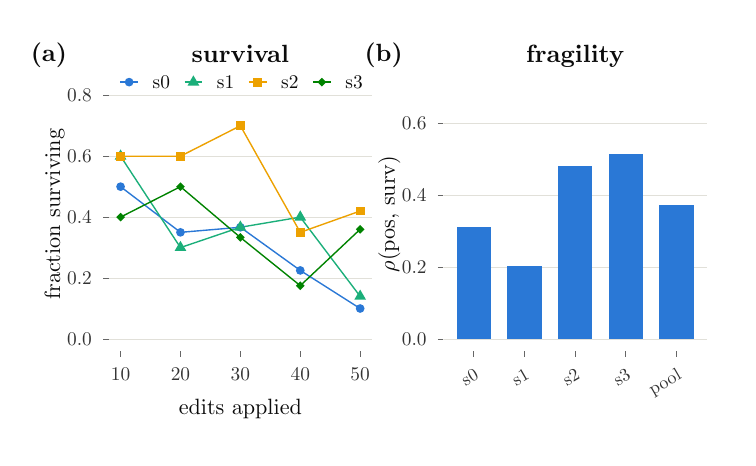
\begin{tikzpicture}[x=1pt,y=1pt]
\definecolor{fillColor}{RGB}{255,255,255}
\path[use as bounding box,fill=fillColor,fill opacity=0.00] (0,0) rectangle (252.94,148.15);
\begin{scope}
\path[clip] (  0.00,  0.00) rectangle (252.94,148.15);
\definecolor{drawColor}{RGB}{255,255,255}
\definecolor{fillColor}{RGB}{255,255,255}

\path[draw=drawColor,line width= 0.6pt,line join=round,line cap=round,fill=fillColor] (  0.00,  0.00) rectangle (252.94,148.15);
\end{scope}
\begin{scope}
\path[clip] (  5.50,  5.50) rectangle (126.47,142.65);
\definecolor{fillColor}{RGB}{255,255,255}

\path[fill=fillColor] (  5.50,  5.50) rectangle (126.47,142.65);
\end{scope}
\begin{scope}
\path[clip] (126.47,  5.50) rectangle (247.44,142.65);
\definecolor{fillColor}{RGB}{255,255,255}

\path[fill=fillColor] (126.47,  5.50) rectangle (247.44,142.65);
\end{scope}
\begin{scope}
\path[clip] ( 29.24, 31.15) rectangle (124.47,130.43);
\definecolor{drawColor}{RGB}{225,224,217}

\path[draw=drawColor,line width= 0.3pt,line join=round] ( 29.24, 35.66) --
	(124.47, 35.66);

\path[draw=drawColor,line width= 0.3pt,line join=round] ( 29.24, 57.68) --
	(124.47, 57.68);

\path[draw=drawColor,line width= 0.3pt,line join=round] ( 29.24, 79.69) --
	(124.47, 79.69);

\path[draw=drawColor,line width= 0.3pt,line join=round] ( 29.24,101.70) --
	(124.47,101.70);

\path[draw=drawColor,line width= 0.3pt,line join=round] ( 29.24,123.72) --
	(124.47,123.72);
\definecolor{drawColor}{RGB}{42,120,214}

\path[draw=drawColor,line width= 0.5pt,line join=round] ( 33.57, 90.70) --
	( 55.21, 74.19) --
	( 76.86, 76.03) --
	( 98.50, 60.43) --
	(120.14, 46.67);
\definecolor{drawColor}{RGB}{27,175,122}

\path[draw=drawColor,line width= 0.5pt,line join=round] ( 33.57,101.70) --
	( 55.21, 68.68) --
	( 76.86, 76.03) --
	( 98.50, 79.69) --
	(120.14, 51.07);
\definecolor{drawColor}{RGB}{237,161,0}

\path[draw=drawColor,line width= 0.5pt,line join=round] ( 33.57,101.70) --
	( 55.21,101.70) --
	( 76.86,112.71) --
	( 98.50, 74.19) --
	(120.14, 81.89);
\definecolor{drawColor}{RGB}{0,131,0}

\path[draw=drawColor,line width= 0.5pt,line join=round] ( 33.57, 79.69) --
	( 55.21, 90.70) --
	( 76.86, 72.35) --
	( 98.50, 54.93) --
	(120.14, 75.29);
\definecolor{fillColor}{RGB}{42,120,214}

\path[fill=fillColor] ( 33.57, 90.70) circle (  1.58);

\path[fill=fillColor] ( 55.21, 74.19) circle (  1.58);

\path[fill=fillColor] ( 76.86, 76.03) circle (  1.58);

\path[fill=fillColor] ( 98.50, 60.43) circle (  1.58);

\path[fill=fillColor] (120.14, 46.67) circle (  1.58);
\definecolor{fillColor}{RGB}{27,175,122}

\path[fill=fillColor] ( 33.57,104.16) --
	( 35.69,100.48) --
	( 31.45,100.48) --
	cycle;

\path[fill=fillColor] ( 55.21, 71.14) --
	( 57.34, 67.46) --
	( 53.09, 67.46) --
	cycle;

\path[fill=fillColor] ( 76.86, 78.48) --
	( 78.98, 74.80) --
	( 74.73, 74.80) --
	cycle;

\path[fill=fillColor] ( 98.50, 82.14) --
	(100.62, 78.47) --
	( 96.38, 78.47) --
	cycle;

\path[fill=fillColor] (120.14, 53.52) --
	(122.27, 49.85) --
	(118.02, 49.85) --
	cycle;
\definecolor{fillColor}{RGB}{237,161,0}

\path[fill=fillColor] ( 31.99,100.13) --
	( 35.14,100.13) --
	( 35.14,103.28) --
	( 31.99,103.28) --
	cycle;

\path[fill=fillColor] ( 53.64,100.13) --
	( 56.79,100.13) --
	( 56.79,103.28) --
	( 53.64,103.28) --
	cycle;

\path[fill=fillColor] ( 75.28,111.13) --
	( 78.43,111.13) --
	( 78.43,114.29) --
	( 75.28,114.29) --
	cycle;

\path[fill=fillColor] ( 96.92, 72.61) --
	(100.08, 72.61) --
	(100.08, 75.76) --
	( 96.92, 75.76) --
	cycle;

\path[fill=fillColor] (118.57, 80.32) --
	(121.72, 80.32) --
	(121.72, 83.47) --
	(118.57, 83.47) --
	cycle;
\definecolor{fillColor}{RGB}{0,131,0}

\path[fill=fillColor] ( 31.99, 79.69) --
	( 33.57, 81.27) --
	( 35.14, 79.69) --
	( 33.57, 78.11) --
	cycle;

\path[fill=fillColor] ( 53.64, 90.70) --
	( 55.21, 92.27) --
	( 56.79, 90.70) --
	( 55.21, 89.12) --
	cycle;

\path[fill=fillColor] ( 75.28, 72.35) --
	( 76.86, 73.93) --
	( 78.43, 72.35) --
	( 76.86, 70.77) --
	cycle;

\path[fill=fillColor] ( 96.92, 54.93) --
	( 98.50, 56.50) --
	(100.08, 54.93) --
	( 98.50, 53.35) --
	cycle;

\path[fill=fillColor] (118.57, 75.29) --
	(120.14, 76.86) --
	(121.72, 75.29) --
	(120.14, 73.71) --
	cycle;
\end{scope}
\begin{scope}
\path[clip] (  0.00,  0.00) rectangle (252.94,148.15);
\definecolor{drawColor}{gray}{0.20}

\node[text=drawColor,anchor=base east,inner sep=0pt, outer sep=0pt, scale=  0.70] at ( 23.19, 33.39) {0.0};

\node[text=drawColor,anchor=base east,inner sep=0pt, outer sep=0pt, scale=  0.70] at ( 23.19, 55.40) {0.2};

\node[text=drawColor,anchor=base east,inner sep=0pt, outer sep=0pt, scale=  0.70] at ( 23.19, 77.41) {0.4};

\node[text=drawColor,anchor=base east,inner sep=0pt, outer sep=0pt, scale=  0.70] at ( 23.19, 99.43) {0.6};

\node[text=drawColor,anchor=base east,inner sep=0pt, outer sep=0pt, scale=  0.70] at ( 23.19,121.44) {0.8};
\end{scope}
\begin{scope}
\path[clip] (  0.00,  0.00) rectangle (252.94,148.15);
\definecolor{drawColor}{gray}{0.40}

\path[draw=drawColor,line width= 0.3pt,line join=round] ( 27.24, 35.66) --
	( 29.24, 35.66);

\path[draw=drawColor,line width= 0.3pt,line join=round] ( 27.24, 57.68) --
	( 29.24, 57.68);

\path[draw=drawColor,line width= 0.3pt,line join=round] ( 27.24, 79.69) --
	( 29.24, 79.69);

\path[draw=drawColor,line width= 0.3pt,line join=round] ( 27.24,101.70) --
	( 29.24,101.70);

\path[draw=drawColor,line width= 0.3pt,line join=round] ( 27.24,123.72) --
	( 29.24,123.72);
\end{scope}
\begin{scope}
\path[clip] (  0.00,  0.00) rectangle (252.94,148.15);
\definecolor{drawColor}{gray}{0.40}

\path[draw=drawColor,line width= 0.3pt,line join=round] ( 33.57, 29.15) --
	( 33.57, 31.15);

\path[draw=drawColor,line width= 0.3pt,line join=round] ( 55.21, 29.15) --
	( 55.21, 31.15);

\path[draw=drawColor,line width= 0.3pt,line join=round] ( 76.86, 29.15) --
	( 76.86, 31.15);

\path[draw=drawColor,line width= 0.3pt,line join=round] ( 98.50, 29.15) --
	( 98.50, 31.15);

\path[draw=drawColor,line width= 0.3pt,line join=round] (120.14, 29.15) --
	(120.14, 31.15);
\end{scope}
\begin{scope}
\path[clip] (  0.00,  0.00) rectangle (252.94,148.15);
\definecolor{drawColor}{gray}{0.20}

\node[text=drawColor,anchor=base,inner sep=0pt, outer sep=0pt, scale=  0.70] at ( 33.57, 20.54) {10};

\node[text=drawColor,anchor=base,inner sep=0pt, outer sep=0pt, scale=  0.70] at ( 55.21, 20.54) {20};

\node[text=drawColor,anchor=base,inner sep=0pt, outer sep=0pt, scale=  0.70] at ( 76.86, 20.54) {30};

\node[text=drawColor,anchor=base,inner sep=0pt, outer sep=0pt, scale=  0.70] at ( 98.50, 20.54) {40};

\node[text=drawColor,anchor=base,inner sep=0pt, outer sep=0pt, scale=  0.70] at (120.14, 20.54) {50};
\end{scope}
\begin{scope}
\path[clip] (  0.00,  0.00) rectangle (252.94,148.15);
\definecolor{drawColor}{RGB}{11,11,11}

\node[text=drawColor,anchor=base,inner sep=0pt, outer sep=0pt, scale=  0.80] at ( 76.86,  8.23) {edits applied};
\end{scope}
\begin{scope}
\path[clip] (  0.00,  0.00) rectangle (252.94,148.15);
\definecolor{drawColor}{RGB}{11,11,11}

\node[text=drawColor,rotate= 90.00,anchor=base,inner sep=0pt, outer sep=0pt, scale=  0.80] at ( 11.71, 80.79) {fraction surviving};
\end{scope}
\begin{scope}
\path[clip] (  0.00,  0.00) rectangle (252.94,148.15);
\definecolor{drawColor}{RGB}{42,120,214}

\path[draw=drawColor,line width= 0.5pt,line join=round] ( 33.46,128.47) -- ( 39.86,128.47);
\definecolor{fillColor}{RGB}{42,120,214}

\path[fill=fillColor] ( 36.66,128.47) circle (  1.58);
\end{scope}
\begin{scope}
\path[clip] (  0.00,  0.00) rectangle (252.94,148.15);
\definecolor{drawColor}{RGB}{27,175,122}

\path[draw=drawColor,line width= 0.5pt,line join=round] ( 56.68,128.47) -- ( 63.08,128.47);
\definecolor{fillColor}{RGB}{27,175,122}

\path[fill=fillColor] ( 59.88,130.92) --
	( 62.01,127.24) --
	( 57.76,127.24) --
	cycle;
\end{scope}
\begin{scope}
\path[clip] (  0.00,  0.00) rectangle (252.94,148.15);
\definecolor{drawColor}{RGB}{237,161,0}

\path[draw=drawColor,line width= 0.5pt,line join=round] ( 79.91,128.47) -- ( 86.31,128.47);
\definecolor{fillColor}{RGB}{237,161,0}

\path[fill=fillColor] ( 81.53,126.89) --
	( 84.68,126.89) --
	( 84.68,130.04) --
	( 81.53,130.04) --
	cycle;
\end{scope}
\begin{scope}
\path[clip] (  0.00,  0.00) rectangle (252.94,148.15);
\definecolor{drawColor}{RGB}{0,131,0}

\path[draw=drawColor,line width= 0.5pt,line join=round] (103.13,128.47) -- (109.53,128.47);
\definecolor{fillColor}{RGB}{0,131,0}

\path[fill=fillColor] (104.75,128.47) --
	(106.33,130.04) --
	(107.91,128.47) --
	(106.33,126.89) --
	cycle;
\end{scope}
\begin{scope}
\path[clip] (  0.00,  0.00) rectangle (252.94,148.15);
\definecolor{drawColor}{RGB}{11,11,11}

\node[text=drawColor,anchor=base west,inner sep=0pt, outer sep=0pt, scale=  0.70] at ( 45.16,126.19) {s0};
\end{scope}
\begin{scope}
\path[clip] (  0.00,  0.00) rectangle (252.94,148.15);
\definecolor{drawColor}{RGB}{11,11,11}

\node[text=drawColor,anchor=base west,inner sep=0pt, outer sep=0pt, scale=  0.70] at ( 68.38,126.19) {s1};
\end{scope}
\begin{scope}
\path[clip] (  0.00,  0.00) rectangle (252.94,148.15);
\definecolor{drawColor}{RGB}{11,11,11}

\node[text=drawColor,anchor=base west,inner sep=0pt, outer sep=0pt, scale=  0.70] at ( 91.61,126.19) {s2};
\end{scope}
\begin{scope}
\path[clip] (  0.00,  0.00) rectangle (252.94,148.15);
\definecolor{drawColor}{RGB}{11,11,11}

\node[text=drawColor,anchor=base west,inner sep=0pt, outer sep=0pt, scale=  0.70] at (114.83,126.19) {s3};
\end{scope}
\begin{scope}
\path[clip] (  0.00,  0.00) rectangle (252.94,148.15);
\definecolor{drawColor}{RGB}{11,11,11}

\node[text=drawColor,anchor=base,inner sep=0pt, outer sep=0pt, scale=  0.90] at ( 76.86,135.45) {\bfseries survival};
\end{scope}
\begin{scope}
\path[clip] (  0.00,  0.00) rectangle (252.94,148.15);
\definecolor{drawColor}{RGB}{11,11,11}

\node[text=drawColor,anchor=base,inner sep=0pt, outer sep=0pt, scale=  0.90] at (  7.68,135.85) {\bfseries (a)};
\end{scope}
\begin{scope}
\path[clip] (150.21, 31.15) rectangle (245.44,130.43);
\definecolor{drawColor}{RGB}{225,224,217}

\path[draw=drawColor,line width= 0.3pt,line join=round] (150.21, 35.66) --
	(245.44, 35.66);

\path[draw=drawColor,line width= 0.3pt,line join=round] (150.21, 61.68) --
	(245.44, 61.68);

\path[draw=drawColor,line width= 0.3pt,line join=round] (150.21, 87.70) --
	(245.44, 87.70);

\path[draw=drawColor,line width= 0.3pt,line join=round] (150.21,113.72) --
	(245.44,113.72);
\definecolor{fillColor}{RGB}{42,120,214}

\path[fill=fillColor] (154.97, 35.66) rectangle (167.43, 76.23);

\path[fill=fillColor] (173.29, 35.66) rectangle (185.74, 61.90);

\path[fill=fillColor] (191.60, 35.66) rectangle (204.06, 98.32);

\path[fill=fillColor] (209.92, 35.66) rectangle (222.37,102.52);

\path[fill=fillColor] (228.23, 35.66) rectangle (240.68, 84.01);
\end{scope}
\begin{scope}
\path[clip] (  0.00,  0.00) rectangle (252.94,148.15);
\definecolor{drawColor}{gray}{0.20}

\node[text=drawColor,anchor=base east,inner sep=0pt, outer sep=0pt, scale=  0.70] at (144.16, 33.39) {0.0};

\node[text=drawColor,anchor=base east,inner sep=0pt, outer sep=0pt, scale=  0.70] at (144.16, 59.40) {0.2};

\node[text=drawColor,anchor=base east,inner sep=0pt, outer sep=0pt, scale=  0.70] at (144.16, 85.42) {0.4};

\node[text=drawColor,anchor=base east,inner sep=0pt, outer sep=0pt, scale=  0.70] at (144.16,111.44) {0.6};
\end{scope}
\begin{scope}
\path[clip] (  0.00,  0.00) rectangle (252.94,148.15);
\definecolor{drawColor}{gray}{0.40}

\path[draw=drawColor,line width= 0.3pt,line join=round] (148.21, 35.66) --
	(150.21, 35.66);

\path[draw=drawColor,line width= 0.3pt,line join=round] (148.21, 61.68) --
	(150.21, 61.68);

\path[draw=drawColor,line width= 0.3pt,line join=round] (148.21, 87.70) --
	(150.21, 87.70);

\path[draw=drawColor,line width= 0.3pt,line join=round] (148.21,113.72) --
	(150.21,113.72);
\end{scope}
\begin{scope}
\path[clip] (  0.00,  0.00) rectangle (252.94,148.15);
\definecolor{drawColor}{gray}{0.40}

\path[draw=drawColor,line width= 0.3pt,line join=round] (161.20, 29.15) --
	(161.20, 31.15);

\path[draw=drawColor,line width= 0.3pt,line join=round] (179.51, 29.15) --
	(179.51, 31.15);

\path[draw=drawColor,line width= 0.3pt,line join=round] (197.83, 29.15) --
	(197.83, 31.15);

\path[draw=drawColor,line width= 0.3pt,line join=round] (216.14, 29.15) --
	(216.14, 31.15);

\path[draw=drawColor,line width= 0.3pt,line join=round] (234.46, 29.15) --
	(234.46, 31.15);
\end{scope}
\begin{scope}
\path[clip] (  0.00,  0.00) rectangle (252.94,148.15);
\definecolor{drawColor}{gray}{0.20}

\node[text=drawColor,rotate= 30.00,anchor=base east,inner sep=0pt, outer sep=0pt, scale=  0.65] at (163.32, 21.44) {s0};

\node[text=drawColor,rotate= 30.00,anchor=base east,inner sep=0pt, outer sep=0pt, scale=  0.65] at (181.63, 21.44) {s1};

\node[text=drawColor,rotate= 30.00,anchor=base east,inner sep=0pt, outer sep=0pt, scale=  0.65] at (199.94, 21.44) {s2};

\node[text=drawColor,rotate= 30.00,anchor=base east,inner sep=0pt, outer sep=0pt, scale=  0.65] at (218.26, 21.44) {s3};

\node[text=drawColor,rotate= 30.00,anchor=base east,inner sep=0pt, outer sep=0pt, scale=  0.65] at (236.57, 21.44) {pool};
\end{scope}
\begin{scope}
\path[clip] (  0.00,  0.00) rectangle (252.94,148.15);
\definecolor{drawColor}{RGB}{11,11,11}

\node[text=drawColor,rotate= 90.00,anchor=base,inner sep=0pt, outer sep=0pt, scale=  0.80] at (132.68, 80.79) {$\rho$(pos, surv)};
\end{scope}
\begin{scope}
\path[clip] (  0.00,  0.00) rectangle (252.94,148.15);
\definecolor{drawColor}{RGB}{11,11,11}

\node[text=drawColor,anchor=base,inner sep=0pt, outer sep=0pt, scale=  0.90] at (197.83,135.45) {\bfseries fragility};
\end{scope}
\begin{scope}
\path[clip] (  0.00,  0.00) rectangle (252.94,148.15);
\definecolor{drawColor}{RGB}{11,11,11}

\node[text=drawColor,anchor=base,inner sep=0pt, outer sep=0pt, scale=  0.90] at (128.65,135.85) {\bfseries (b)};
\end{scope}
\end{tikzpicture}
